% Chapter Template

% Main chapter title
%\chapter[toc version]{doc version}
\chapter{Background}

% Short version of the title for the header
%\chaptermark{version for header}

% Chapter Label
% For referencing this chapter elsewhere, use \ref{ChapterTemplate}
\label{chp:background}

% Write text in here
% Use \subsection and \subsubsection to organize text

\algdef{SE}[SUBALG]{Indent}{EndIndent}{}{\algorithmicend\ }%
\algtext*{Indent}
\algtext*{EndIndent}

\section{Introduction}
\label{sec:background_intro}
We will use deep neural networks and probabilistic models extensively throughout this thesis. Although the basic concepts of the former should be fairly familiar to most readers, the latter might be less widely known. Moreover, some of the tools and algorithms that we are going to use are not so trivial and therefore they should better be introduced first, for the sake of completeness and readability.

This chapter will then focus on providing a brief yet rigorous background on the aforementioned subject. We shall start by clarifying some notations and conventions we shall adopt (\Secref{sec:definitions}). Then we proceed with a short introduction to Bayesian networks, motivated by the factorization properties of joint probability functions (\Secref{}). Expectation-Maximization (EM) is presented as an efficient algorithm to learn probabilistic models with unobserved variables (\Secref{}). We then review the hidden Markov model (HMM), which will play a central role in Chapter \ref{chp:networked_data_streams}, and present the instantiation of the EM algorithm for this particular model (\Secref{}). The chapter is concluded with a brief introduction to variational inference (\Secref{}). Under this setting, the variational autoencoder will deserve special attention (\Secref{}), as it will be one of the models employed in Chapter \ref{chp:domain_generalization}.

\section{Useful definitions and conventions}
\label{sec:definitions}
In this section, we introduce some further notations and definitions that will be used throughout this document.

It is important to remark that the same notation is used to denote discrete and continuous random variables as well as to denote probability mass functions and probability density functions. Specifically, given a random variable $\rx$ taking values in the set $\mathrm{Val}(\rx)$, $p(\rx)$ denotes the probability mass of $\rx$, if $\mathrm{Val}(\rx)$ is discrete, or the probability density of $\rx$, otherwise. In either case, the \emph{support} of $p(\rx)$ is defined as $\mathrm{Supp}(p(\rx)) \triangleq \lbrace x \in \mathrm{Val}(\rx): p(\rx=x) > 0 \rbrace$. Moreover, when we want to denote the probability (density) of some arbitrary but fixed value $x \in \mathrm{Val}(\rx)$, we often use $p(x)$ as a short for $p(\rx=x)$.

The joint probability function of $\rx$ and $\ry$ is denoted by $p(\rx,\ry)$ and the corresponding conditionals of $\ry$ given $\rx$ and $\rx$ given $\ry$ are denoted by the usual $p(\ry \mid \rx)$ and $p(\rx \mid \ry)$, respectively. Again, $\rx$ and $\ry$ can be both discrete, both continuous, or one continuous and the other discrete. For three or more random variables the notation generalizes naturally.

The marginalization of $p(\rx,\ry)$ with respect to a discrete $\ry$ is written as:
\begin{equation}
    \sum_{\ry} p(\rx,\ry) \triangleq \sum_{y \in \mathrm{Val}(\ry)} p(\rx,y) = p(\rx),
\end{equation}
and the marginalization of $p(\rx,\ry)$ with respect to a continuous $\rx$ is written as:
\begin{equation}
    \int p(\rx,\ry) \d \rx \triangleq \int_{\mathrm{Val}(\rx)} p(x,\ry) \d x = p(\ry).
\end{equation}
Note that for brevity we omit the domain of the summation or integration, as this is defined implicitly by the set where the random variable is defined. The integral notation is also used for the marginalization with respect to random variables whose type is unspecified. Similarly, if $f(\rx)$ is a function of a random variable $\rx$,
\begin{equation}
    \sum_\rx f(\rx) \triangleq \sum_{x \in \mathrm{Val}(\rx)} f(x) \quad \text{or} \quad \int f(\rx) \d \rx \triangleq \int_{\mathrm{Val}(\rx)} f(x) \d x,
\end{equation}
depending on whether $\rx$ is discrete or continuous, respectively. Hence, we can write the \emph{expectation} of $f(\rx)$ with respect to $p(\rx)$ as:
\begin{equation}
    \E_{\rx \sim p(\rx)} \left[f(\rx)\right] \triangleq \sum_\rx f(\rx) p(\rx) \quad \text{or} \quad \E_{\rx \sim p(\rx)} \left[f(\rx)\right] \triangleq \int f(\rx) p(\rx) \d \rx,
\end{equation}
for a discrete or continuous $\rx$, respectively.

\section{Bayesian networks}
\label{sec:bayesian_networks}

\subsection{Definition and structural properties}
\label{sec:bayesian_net_definition}

Given $m$ random variables $\rx_1, \rx_2, \dots, \rx_m$, the \emph{chain rule of probability} allows the factorization of their joint distribution as a product of conditional distributions:\footnote{The expression on the right-hand side of \eqref{eq:chain_rule} is not well defined outside the support of $p(\rx^{(1)}), p(\rx^{(1)}, \rx^{(2)}), \dots, p(\rx^{(1)}, \rx^{(2)}, \dots, \rx^{(m-1)})$. For those values, one has $p(\rx^{(1)}, \rx^{(2)}, \dots, \rx^{(m)})=0$.}
\begin{equation}
    \label{eq:chain_rule}
    p(\rx^{(1)},\rx^{(2)},\dots,\rx^{(m)}) = p(\rx^{(1)}) \prod_{j=1}^m p(\rx^{(j)} \mid \rx^{(1)}, \rx^{(2)}, \dots, \rx^{(j-1})).
\end{equation}
Starting from a factorization of a joint distribution into conditionals, we may build a directed graph $\gG$ with $m$ vertices, one for each random variable, where there exists an edge $i \rightarrow j$ if and only if there is a factor where $\rx^{(j)}$ is conditioned on $\rx^{(i)}$. Such a graph is known as a \emph{Bayesian network}. From its definition, we see that the factorization in \eqref{eq:chain_rule} corresponds to the graph in \Figref{fig:complete_bayesian_net}. Clearly, a Bayesian network defines a bijection between random variables and graph nodes, so with a slight abuse of terminology we represent and refer to nodes by the random variable they are associated with, rather than by their index.

\begin{figure}
    \centering
    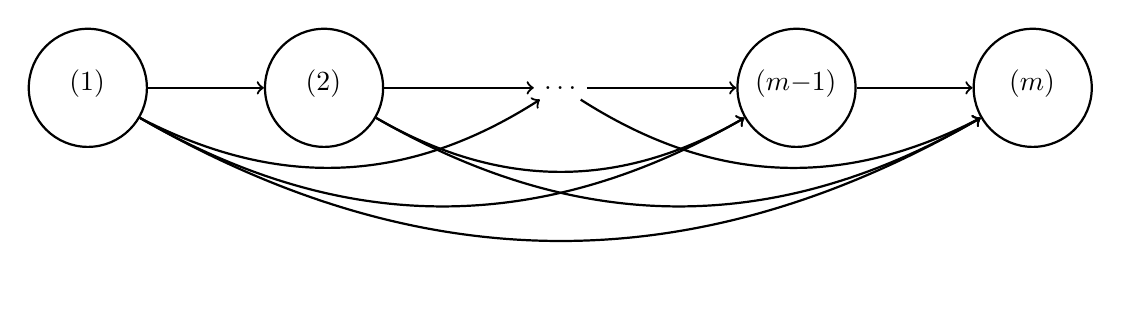
\begin{tikzpicture}[auto, node distance=3cm, every loop/.style={},thick,
        main node/.style={circle,draw,font=\sffamily\Large\bfseries},
        hidden node/.style={circle,draw,fill=lightgray,font=\sffamily\Large\bfseries},
        box node/.style={rectangle,dashed,draw,anchor=center},
        empty node/.style={rectangle,fill=white,anchor=center},]


        \node[main node,minimum size=1.5cm] (x1) {$\rx^{(1)}$};
        \node[main node,minimum size=1.5cm] (x2) [right of=x1] {$\rx^{(2)}$};
        \node[empty node] (dots) [right of=x2] {$\dots$};
        \node[main node,minimum size=1.5cm] (xm_1) [right of=dots] {$\rx^{(m-1)}$};
        \node[main node,minimum size=1.5cm] (xm) [right of=xm_1] {$\rx^{(m)}$};


        \draw[->]
        (x1) edge (x2)
        (x2) edge (dots)
        (dots) edge (xm_1)
        (xm_1) edge (xm)
        (x1) edge[bend right] (dots)
        (x1) edge[bend right] (xm)
        (x1) edge[bend right] (xm_1)
        (x2) edge[bend right] (xm_1)
        (x2) edge[bend right] (xm)
        (dots) edge[bend right] (xm);

    \end{tikzpicture}
    \caption{A complete Bayesian network.}
    \label{fig:complete_bayesian_net}
\end{figure}

Since the factorization in \eqref{eq:chain_rule} is general (i.e.\ it does not assume any conditional independencies between random variables), the Bayesian network in \Figref{fig:complete_bayesian_net} is said to be \emph{complete}. When conditional independencies are present, the graph becomes sparser. For instance, if, for all $j \geq 3$, $\rx^{(j)}$ is conditionally independent of $\rx^{(1)}, \rx^{(2)}, \dots, \rx^{(j-2)}$ given $\rx^{(j-1)}$, then $p(\rx^{(j)} \mid \rx^{(1)}, \rx^{(2)}, \dots, \rx^{(j-1)}) = p(\rx^{(j)} \mid \rx^{(j-1)})$ and thus the Bayesian network reduces to the \emph{chain} represented in \Figref{fig:chain_bayesian_net}. A sparser graph implies a more compact parametrization of the model. For instance, if each of the $m$ random variables takes values on a discrete set of size $s$, defining the joint distribution corresponding to a complete Bayesian network (\Figref{fig:complete_bayesian_net}) would require $s^{m}-1$ parameters. However, in the same setting, the joint distribution corresponding to a chain (\Figref{fig:chain_bayesian_net}) can be fully described using table conditional probability distributions (CPDs) with less than $s^2m$ parameters in total.

\begin{figure}
    \centering
    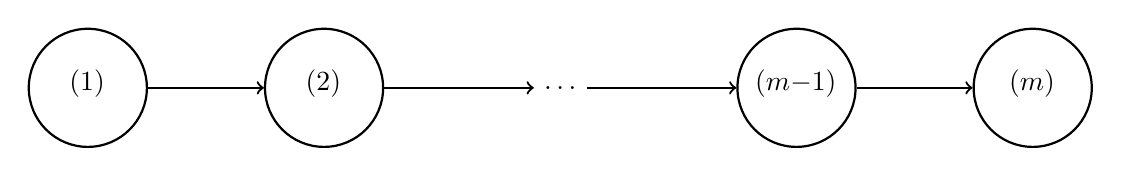
\begin{tikzpicture}[auto, node distance=3cm, every loop/.style={},thick,
        main node/.style={circle,draw,font=\sffamily\Large\bfseries},
        hidden node/.style={circle,draw,fill=lightgray,font=\sffamily\Large\bfseries},
        box node/.style={rectangle,dashed,draw,anchor=center},
        empty node/.style={rectangle,fill=white,anchor=center},]


        \node[main node,minimum size=1.5cm] (x1) {$\rx^{(1)}$};
        \node[main node,minimum size=1.5cm] (x2) [right of=x1] {$\rx^{(2)}$};
        \node[empty node] (dots) [right of=x2] {$\dots$};
        \node[main node,minimum size=1.5cm] (xm_1) [right of=dots] {$\rx^{(m-1)}$};
        \node[main node,minimum size=1.5cm] (xm) [right of=xm_1] {$\rx^{(m)}$};


        \draw[->]
        (x1) edge (x2)
        (x2) edge (dots)
        (dots) edge (xm_1)
        (xm_1) edge (xm);;
    \end{tikzpicture}
    \caption{A chain.}
    \label{fig:chain_bayesian_net}
\end{figure}
An important property of Bayesian networks is the fact that they are always directed \emph{acyclic} graphs. The non-existence of cycles allows us to recover the factorization of the joint distribution by examining the structure of the graph $\gG$ and applying the formula:
\begin{equation}
    p(\rx^{(1)}, \rx^{(2)}, \dots, \rx^{(n)}) = \prod_{j=1}^m p(\rx^{(j)} \mid \parents_\gG(\rx^{(j)})),
\end{equation}
where $\parents_\gG(\rx^{(j)})$ are the parents of node $\rx^{(j)}$ in $\gG$. It is important to highlight that, although there is a one-to-one correspondence between a factorization of a joint distribution into conditional distributions and a Bayesian network, the same joint distribution can sometimes be factorized in multiple different but equivalent forms, each one corresponding to a different Bayesian network. Note, for instance, that \eqref{eq:chain_rule} is just one out of $m!$ possible ways of factorizing $p(\rx^{(1)},\rx^{(2)},\dots,\rx^{(m)})$ using the chain rule and any of those factorizations would yield a different graph. This is also the case for chains and \emph{forks}, which we discuss next.

\subsection{Chains and forks}
\label{sec:chains_forks}
Let us consider the case where we have three random variables $\rx^{(1)}, \rx^{(2)}, \rx^{(3)}$ and assume that $\rx^{(1)}$ and $\rx^{(3)}$ are independent given $\rx^{(2)}$. Under this setting, we have:
\begin{align}
    p(\rx^{(1)}, \rx^{(2)}, \rx^{(3)}) &= p(\rx^{(1)}) p(\rx^{(2)} \mid \rx^{(1)}) p(\rx^{(3)} \mid \rx^{(2)}) \label{eq:chain}\\
    &= p(\rx^{(2)}) p(\rx^{(1)} \mid \rx^{(2)}) p(\rx^{(3)} \mid \rx^{(2)}) \label{eq:fork}\\
    &= p(\rx^{(3)}) p(\rx^{(2)} \mid \rx^{(3)}) p(\rx^{(1)} \mid \rx^{(2)}) \label{eq:reversed_chain}
\end{align}
The three equivalent factorizations \plaineqref{eq:chain} -- \plaineqref{eq:reversed_chain} correspond to the three Bayesian networks in \Figref{fig:equiv_bayesian_nets}, respectively from left to right.

\begin{figure}
    \centering
    \begin{subfigure}[t]{0.32\textwidth}
        \resizebox{\textwidth}{!}{
        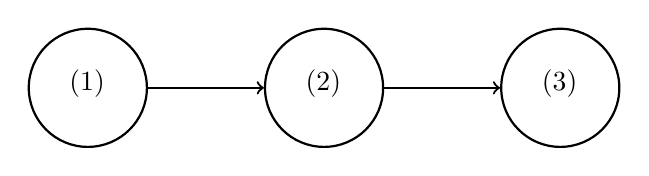
\begin{tikzpicture}[auto, node distance=3cm, every loop/.style={},thick,
            main node/.style={circle,draw,font=\sffamily\Large\bfseries},
            hidden node/.style={circle,draw,fill=lightgray,font=\sffamily\Large\bfseries},
            box node/.style={rectangle,dashed,draw,anchor=center},
            empty node/.style={rectangle,fill=white,anchor=center},]


            \node[main node,minimum size=1.5cm] (x1) {$\rx^{(1)}$};
            \node[main node,minimum size=1.5cm] (x2) [right of=x1] {$\rx^{(2)}$};
            \node[main node,minimum size=1.5cm] (x3) [right of=x2] {$\rx^{(3)}$};

            \draw[->]
            (x1) edge (x2)
            (x2) edge (x3);
        \end{tikzpicture}}
        \caption{A three-variable chain.}
        \label{fig:3var_chain_bayesian_net}
    \end{subfigure}
    \begin{subfigure}[t]{0.32\textwidth}
        \resizebox{\textwidth}{!}{
        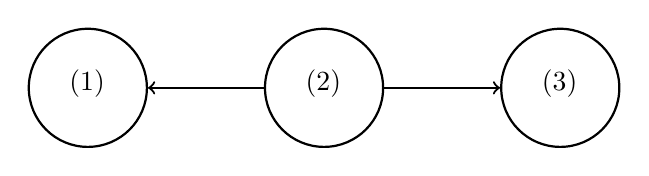
\begin{tikzpicture}[auto, node distance=3cm, every loop/.style={},thick,
            main node/.style={circle,draw,font=\sffamily\Large\bfseries},
            hidden node/.style={circle,draw,fill=lightgray,font=\sffamily\Large\bfseries},
            box node/.style={rectangle,dashed,draw,anchor=center},
            empty node/.style={rectangle,fill=white,anchor=center},]
            \node[main node,minimum size=1.5cm] (x1) {$\rx^{(1)}$};
            \node[main node,minimum size=1.5cm] (x2) [right of=x1] {$\rx^{(2)}$};
            \node[main node,minimum size=1.5cm] (x3) [right of=x2] {$\rx^{(3)}$};
            \draw[->]
            (x2) edge (x1)
            (x2) edge (x3);
        \end{tikzpicture}}
        \caption{A fork.}
        \label{fig:fork_bayesian_net}
    \end{subfigure}
    \begin{subfigure}[t]{0.32\textwidth}
        \resizebox{\textwidth}{!}{
        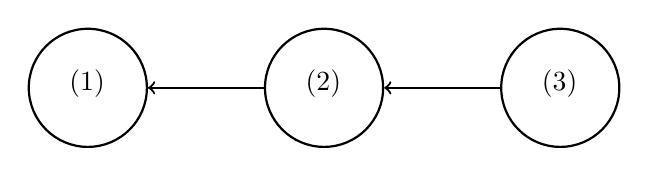
\begin{tikzpicture}[auto, node distance=3cm, every loop/.style={},thick,
            main node/.style={circle,draw,font=\sffamily\Large\bfseries},
            hidden node/.style={circle,draw,fill=lightgray,font=\sffamily\Large\bfseries},
            box node/.style={rectangle,dashed,draw,anchor=center},
            empty node/.style={rectangle,fill=white,anchor=center},]


            \node[main node,minimum size=1.5cm] (x1) {$\rx^{(1)}$};
            \node[main node,minimum size=1.5cm] (x2) [right of=x1] {$\rx^{(2)}$};
            \node[main node,minimum size=1.5cm] (x3) [right of=x2] {$\rx^{(3)}$};

            \draw[->]
            (x3) edge (x2)
            (x2) edge (x1);
        \end{tikzpicture}}
        \caption{A three-variable reversed chain.}
        \label{fig:revchain_bayesian_net}
    \end{subfigure}
    \caption{Equivalent three-variable Bayesian networks.}
    \label{fig:equiv_bayesian_nets}
\end{figure}

\subsection{Immoralities}
\label{sec:immoralities}
Now let us assume that $\rx^{(1)}$ and $\rx^{(3)}$ are marginally independent, which notably does not imply that they are conditionally independent given $\rx^{(2)}$. In this case, the joint distribution factorizes as:
\begin{equation}
    p(\rx^{(1)}, \rx^{(2)}, \rx^{(3)}) = p(\rx^{(1)}) p(\rx^{(3)}) p(\rx^{(2)} \mid \rx^{(1)}, \rx^{(3)})
\end{equation}
and this factorization is unique in the sense that no other implies the same set of conditional independencies. The corresponding Bayesian network is represented in \Figref{fig:immorality_bayesian_net}. A subgraph consisting of three nodes where two of them are not  connected and the other one is a child of both is an \emph{immorality}. The node where the two incoming edges coincide is a \emph{collider}. Thus, in the present example, $\rx^{(1)}$, $\rx^{(2)}$, and $\rx^{(3)}$ form an immorality where $\rx^{(2)}$ is the collider.

\begin{figure}
    \centering
    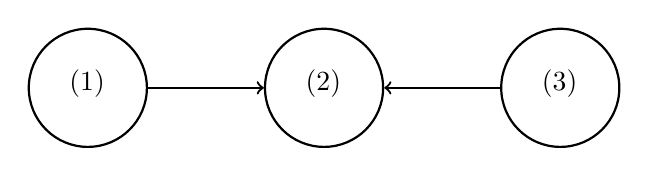
\begin{tikzpicture}[auto, node distance=3cm, every loop/.style={},thick,
        main node/.style={circle,draw,font=\sffamily\Large\bfseries},
        hidden node/.style={circle,draw,fill=lightgray,font=\sffamily\Large\bfseries},
        box node/.style={rectangle,dashed,draw,anchor=center},
        empty node/.style={rectangle,fill=white,anchor=center},]


        \node[main node,minimum size=1.5cm] (x1) {$\rx^{(1)}$};
        \node[main node,minimum size=1.5cm] (x2) [right of=x1] {$\rx^{(2)}$};
        \node[main node,minimum size=1.5cm] (x3) [right of=x2] {$\rx^{(3)}$};

        \draw[->]
        (x1) edge (x2)
        (x3) edge (x2);
    \end{tikzpicture}
    \caption{An immorality.}
    \label{fig:immorality_bayesian_net}
\end{figure}

\subsection{D-separation}
\label{sec:d_separation}
Armed with the notions of chains, forks, and immoralities, and the conditional independencies implied by them, we are ready to introduce the concept of \emph{blocked paths} and \emph{d-separation}. The latter provides a powerful graphical method to discover all the conditional independencies implied by any Bayesian network.

Specifically, we say that an undirected path between two nodes $\rx$ and $\ry$ is \emph{blocked} by a (potentially empty) conditioning set $\gS$ if at least one of the following two conditions holds:
\begin{itemize}
    \item Along the path there is a chain or a fork which includes at least one node in $\gS$.
    \item Along the path there is a collider and neither the collider nor any of its descendants are in $\gS$.
\end{itemize}
The two nodes $\rx$ and $\ry$ are \emph{d-separated} by a set of nodes $\gS$ if conditioning on $\gS$ blocks all paths between $\rx$ and $\ry$. Remarkably, if $\rx$ and $\ry$ are d-separated by $\gS$, then they are conditionally independent given $\gS$ (see \citet{Koller2009} for a proof).

\subsection{The hidden Markov model}
\label{sec:hmm}
A classical example of a Bayesian network is the hidden Markov model, represented in \Figref{fig:hmm_bayesian_net}. The HMM will be the backbone of both models presented in Chapter \ref{chp:networked_data_streams} and hence it is appropriate to introduce it here.

\begin{figure}
    \centering
    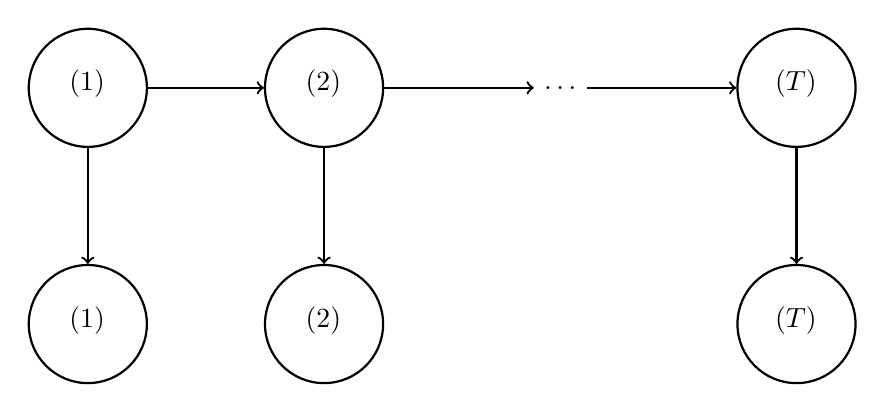
\begin{tikzpicture}[auto, node distance=3cm, every loop/.style={},thick,
        main node/.style={circle,draw,font=\sffamily\Large\bfseries},
        hidden node/.style={circle,draw,fill=lightgray,font=\sffamily\Large\bfseries},
        box node/.style={rectangle,dashed,draw,anchor=center},
        empty node/.style={rectangle,fill=white,anchor=center},]

        \node[main node,minimum size=1.5cm] (h1) {$\rh^{(1)}$};
        \node[main node,minimum size=1.5cm] (h2) [right of=h1] {$\rh^{(2)}$};
        \node[empty node] (dots) [right of=h2] {$\dots$};
        \node[main node,minimum size=1.5cm] (ht) [right of=dots] {$\rh^{(T)}$};
        \node[main node,minimum size=1.5cm] (x1) [below of=h1] {$\rx^{(1)}$};
        \node[main node,minimum size=1.5cm] (x2) [below of=h2] {$\rx^{(2)}$};
        \node[main node,minimum size=1.5cm] (xt) [below of=ht] {$\rx^{(T)}$};


        \draw[->]
        (h1) edge (h2)
        (h2) edge (dots)
        (dots) edge (ht)
        (h1) edge (x1)
        (h2) edge (x2)
        (ht) edge (xt);

    \end{tikzpicture}
    \caption{Hidden Markov model represented as Bayesian network.}
    \label{fig:hmm_bayesian_net}
\end{figure}

The structure of the graph in \Figref{fig:hmm_bayesian_net} corresponds to the following factorization:
\begin{equation}
    p(\rx^{(1)},\rx^{(2)},\dots,\rx^{(T)},\rh^{(1)},\rh^{(2)},\dots,\rh^{(t)}) = p(\rh^{(1)}) p(x^{(1)} \mid h^{(1)}) \prod_{t=2}^T p(h^{(t)} \mid h^{(t-1)}) p(x^{(t)} \mid h^{(t)})
\end{equation}
Here, $\rx^{(1)},\rx^{(2)},\dots,\rx^{(T)}$ is the sequence of \emph{observations} and $\rh^{(1)},\rh^{(2)},\dots,\rh^{(T)}$ is the sequence of \emph{hidden states}.\footnote{The word \emph{hidden} refers to the fact that the states are usually not observed in the training data.} Observations can be either discrete or continuous, while hidden states are usually discrete, although continuous state versions exist (\citet{Turin2004}).

By analyzing d-separation in \Figref{fig:hmm_bayesian_net}, two fundamental assumptions of the HMM are revealed:
\begin{itemize}
    \item For all $t$, the hidden state $\rh^{(t)}$ is conditionally independent of all past hidden states $\rh^{(1)},\rh^{(2)},\dots,\rh^{(t-2)}$ given the previous hidden state $\rh^{(t-1)}$ --- \emph{Markov} assumption.
    \item For all $t$, the observation $\rx^{(t)}$ is conditionally independent of all past and future observations $\rx^{(1)},\dots,\rx^{(t-1)},\rx^{(t+1)},\dots,\rx^{(T)}$ and of all past and future hidden states $\rh^{(1)},\dots,\rh^{(t-1)},\rh^{(t+1)},\dots,\rh^{(T)}$ given the current hidden state $\rh^{(t)}$ --- \emph{output independence} assumption.
\end{itemize}
Furthermore, it is also assumed that both the state transition distribution $p(\rh^{(t)} \mid \rh^{(t-1)})$ and the emission distribution $p(\rx^{(t)} \mid \rh^{(t)})$ are \emph{stationary}, i.e.\ they are the same for all $t$. Besides reducing the number of parameters required to describe the model, the stationarity assumption allows the model to work with sequences of arbitrary length $T$. It should be noted that, in some applications, these assumptions are relaxed yielding HMMs where the hidden state depends on the $k$ previous hidden states ($k$-th order HMM) or where the distributions are time-dependent (non-stationary HMM).

The independence assumptions of the HMM also have the advantage of making inference in this model a tractable problem. Here, we will be particularly interested in computing $p(\rx^{(1)}, \rx^{(2)}, \dots, \rx^{(T)})$, $p(\rh^{(t)} \mid \rvx^{(1)}, \rvx^{(2)}, \dots, \rx^{(T)})$, and $p(\rh^{(t-1)}, \rh^{(t)}  \mid \rx^{(1)}, \rx^{(2)}, \dots, \rx^{(T)})$, which can be obtained with \Algref{alg:forward_backward} (see \citet{Bishop2006} for the derivation).

\begin{algorithm}
    \caption{Forward-backward algorithm (\citet{Rabiner1986}).}
    \label{alg:forward_backward}
    \begin{algorithmic}[1]
        \State \textbf{Inputs:} An observation sequence $x^{(1)}, x^{(2)}, \dots, x^{(T)}$ and an HMM with defined initial state, state transition, and emission distributions.
        \vspace{0.3cm}
        \State Initialize $\alpha_h(1) \coloneqq p(\rh^{(1)}=h)p(x^{(1)} \mid \rh^{(1)}=h)$ and $\beta_h(T) \coloneqq 1$ for all $h$ in the state dictionary.
        \vspace{0.3cm}
        \State Compute the forward recursion $\alpha_h(t) \coloneqq p(x^{(t)} \mid \rh^{(t)}=h) \sum_{\rh^{(t-1)}} \alpha_{\rh^{(t-1)}}(t-1) p(\rh^{(t)}=h \mid \rh^{(t-1)})$ for all $h$ in the state dictionary and $t=2, 3, \dots, T$.
        \vspace{0.3cm}
        \State Compute the backward recursion $\beta_h(t) \coloneqq p(x^{(t+1)} \mid \rh^{(t+1)}=h) \sum_{\rh^{(t+1)}} \beta_{\rh^{(t+1)}}(t+1) p(\rh^{(t+1)} \mid \rh^{(t)}=h) $ for all $h$ in the state dictionary and $t=T-1, T-2, \dots, 1$.
        \vspace{0.3cm}
        \State Obtain the marginal likelihood of the observed sequence as $p(x^{(1)}, x^{(2)}, \dots, x^{(T)}) \coloneqq \sum_{\rh^{(T)}} \alpha_{\rh^{(T)}}(T)$.
        \vspace{0.3cm}
        \State Obtain the state posterior distribution as $p(\rh^{(t)}=h \mid x^{(1)}, x^{(2)}, \dots, x^{(T)}) = \frac{\alpha_h(t)\beta_h(t)}{p(x^{(1)}, x^{(2)}, \dots, x^{(T)})}$ for all $h$ in the state dictionary.
        \vspace{0.3cm}
        \State Obtain the joint posterior distribution of two consecutive states as $p(\rh^{(t-1)}=h, \rh^{(t)}=h' \mid x^{(1)}, x^{(2)}, \dots, x^{(T)}) = \frac{\alpha_h(t-1)p(\rh^{(t)}=h' \mid \rh^{(t-1)}=h) p(x^{(t)} \mid \rh^{(t)}=h')\beta_{h'}(t)}{p(x^{(1)}, x^{(2)}, \dots, x^{(T)})}$ for all $h,h'$ in the state dictionary.
    \end{algorithmic}
\end{algorithm}

\section{The Expectation-Maximization algorithm}
\label{sec:expectation_maximization}

\subsection{General formulation}
\label{sec:general_em}
Given a dataset $\lbrace \vx_i \rbrace_{i=1}^n$ and a probabilistic model with $m$ random variables, the parameters $\Theta$ of the model are often estimated using the \emph{maximum likelihood criterion}, i.e.\ the optimal parameters maximize:
\begin{equation}
    \label{eq:maximum_likelihood}
    J(\Theta) \triangleq \sum_{i=1}^n \log p(\vx_i; \Theta).
\end{equation}
When every example $\vx_i$ is a vector containing an observation for each of the $m$ random variables in the model and $p$ is a usual family of distributions (e.g.\ exponential family or table CPD), objective \plaineqref{eq:maximum_likelihood} is concave and therefore it has a unique maximizer $\Theta^*$. For instance, when $\Theta$ corresponds to the parameters of table CPDs, $\Theta^*$ is given by the empirical conditional probabilities obtained from the provided dataset (see \citet{Koller2009} for a proof).

However, if there exist $\vx_i$ which do not contain observations for some of the $m$ random variables, the maximum likelihood objective becomes non-concave and admits multiple local optima. A procedure to find one of those optimum values is (stochastic) gradient ascent over the likelihood function. A usually better alternative is the Expectation-Maximization algorithm, explained next, since it exhibits faster convergence.

For simplicity, assume that if a random variable is observed in a given example $\vx_i$ then it is observed in all remaining $n-1$ examples as well, i.e.\ assume that the $m$ random variables can be partitioned as $\lbrace \rx^{(j)} \rbrace_{j=1}^o \cup \lbrace \rz^{(j)} \rbrace_{j=1}^l$ where the $\rx^{(j)}$ are the $o$ observed variables and the $\rz^{(j)}$ are the $l$ unobserved (or \emph{latent}) variables and $o+l=m$.\footnote{This assumption is not necessary for the EM algorithm to be valid. However, it makes the exposition simpler and it will hold for all latent variable models considered in this thesis.} Let $\rvx \triangleq \left(\rx^{(1)}, \dots, \rx^{(o)} \right)$ and $\rvz \triangleq \left(\rz^{(1)}, \dots, \rz^{(l)} \right)$ be the vectors of observed and latent variables, respectively. Under this setting, objective \plaineqref{eq:maximum_likelihood} becomes:
\begin{align}
    \label{eq:maximum_marginal_likelihood}
    J(\Theta) &= \sum_{i=1}^n \log \int p(\vx_i, \rvz; \Theta) \d \rvz.
\end{align}
Now, let $q(\rz)$ be an arbitrary distribution such that $\mathrm{Supp}(q(\rvz)) \supseteq \mathrm{Supp}(p(\rvz \mid \vx_i; \Theta))$ for all $i$. Then,
\begingroup
\allowdisplaybreaks
\begin{align}
    J(\Theta) &= \sum_{i=1}^n \log \int \frac{p(\vx_i, \rvz; \Theta)}{q(\rvz)} q(\rvz) \d \rvz \nonumber\\
    &= \sum_{i=1}^n \log \E_{\rvz \sim q} \left[ \frac{p(\vx_i, \rvz; \Theta)} {q(\rvz)} \right] \nonumber\\
    &\geq \sum_{i=1}^n \E_{\rvz \sim q} \left[ \log  \frac{p(\vx_i, \rvz; \Theta)}{q(\rvz)} \right] \triangleq \mathrm{ELBO}(q,\Theta),
\end{align}
\endgroup
where the inequality is a particular case of Jensen's inequality. The EM algorithm proceeds maximizes this \emph{evidence lower bound} (ELBO) in the following block coordinate ascent manner, until a convergence criterion is satisfied:
\begin{itemize}
    \item Keep $\Theta = \Theta^{(-)}$ (fixed) and find $q^* = \argmax_q \mathrm{ELBO}(q, \Theta^{(-)})$ --- \emph{E-step}.
    \item Keep $q = q^{(-)}$ (fixed) and find $\Theta^* = \argmax_\Theta \mathrm{ELBO}(q^{(-)}, \Theta)$ --- \emph{M-step}.
\end{itemize}

\subsection{E-step}
\label{sec:e_step}
Maximizing the ELBO with respect to $q$ is obviously equivalent to the minimization of the difference $J(\Theta^{(-)}) - \mathrm{ELBO}(q, \Theta^{(-)})$ with respect to the same distribution. It is easy to verify that:
\begin{equation}
    J(\Theta^{(-)}) - \mathrm{ELBO}(q, \Theta^{(-)}) = \sum_{i=1}^n \E_{\rvz \sim q} \left[ \log \frac{q(\rvz)}{p(\rvz \mid \vx_i; \Theta^{(-)})} \right] = \KL(q(\rvz) \Vert p(\rvz \mid \vx_i; \Theta^{(-)})),
\end{equation}
where $\KL(q(\rvz) \Vert p(\rvz \mid \vx_i; \Theta^{(-)}))$ denotes the Kullback-Leibler divergence between the distributions $q(\rvz)$ and $p(\rvz \mid \vx_i; \Theta^{(-)})$. This quantity is always non-negative, being zero if and only if the two distributions coincide. Thus, the optimal $q$ is $q^*(\rvz) = p(\rvz \mid \vx_i; \Theta^{(-)})$.

\subsection{M-step}
\label{sec:m_step}
Having found the optimal $q$, we now maximize the ELBO with respect to the parameters $\Theta$. Plugging in $q^{(-)}(z) = p(\rvz \mid \vx_i; \Theta^{(-)})$ yields:
\begin{equation}
    \mathrm{ELBO}(q^{(-)}, \Theta) = \sum_{i=1}^n \E_{\rvz \sim p(\rvz \mid \vx_i; \Theta^{(-)})} \left[ \log p(\vx_i, \rvz; \Theta) \right] - \sum_{i=1}^n \E_{\rvz \sim p(\rvz \mid \vx_i; \Theta^{(-)})} \left[ \log p(\rvz \mid \vx_i; \Theta^{(-)}) \right],
\end{equation}
where the second term is constant with respect to $\Theta$ and therefore can be discarded. The first term is often concave and the maximizer $\Theta^*$ can be written in closed form. This is for instance the case for table CPDs, whose closed-form EM update equations are described next.

\subsection{EM for table CPDs}
\label{sec:em_table_cpd}
We now provide the E-step and M-step update equations applicable to any Bayesian network $\gG$ whose conditional distributions are described by table CPDs. The derivation of these formulas can be found in \citet{Koller2009}.

\paragraph{E-step:} At this stage, using the parameters $\Theta^{(-)}$ obtained at the previous M-step (or the initial parameters if at the beginning), we should obtain the \emph{expected sufficient statistics}. For this purpose, for each random variable $\rw$ in the Bayesian network $\gG$ and for each $(w,\vv) \in \mathrm{Val}(\rw,\parents_\gG(\rw))$:
\begin{itemize}
    \item Compute the posterior distributions $p(\rw,\parents_\gG(\rw) \mid \vx_i; \Theta^{(-)})$ and $p(\parents_\gG(\rw) \mid \vx_i; \Theta^{(-)})$ for each $i$.
    \item Compute the expected sufficient statistics as:
     \begin{align}
         &M(w,\vv) \triangleq \sum_{i=1}^n p(w,\vv \mid \vx_i; \Theta^{(-)}), \label{eq:joint_suf_stat}\\
         &M(\vv) \triangleq \sum_{i=1}^n p(\vv \mid \vx_i; \Theta^{(-)}). \label{eq:marginal_suf_stat}
     \end{align}
\end{itemize}

\paragraph{M-step:} Now, given the expected sufficient statistics computed at the previous E-step, we update the parameters $\Theta$ using:
\begin{equation}
    \theta_{w \mid \vv} = \frac{M(w,\vv)}{M(\vv)},
\end{equation}
where $\theta_{w \mid \vv}$ denotes the table entry corresponding to the probability $p(\rw=w \mid \parents_\gG(\rw)=\vv)$. The set $\Theta$ is the union of all these parameters.

\subsection{EM for the discrete emission HMM}
An example of a table CPD model with latent variables is the HMM with discrete emission distribution. Under this setting, the hidden state $\rh^{(t)}$ and the observation $\rx^{(t)}$ both take values in discrete and finite sets. Thus, we can use \twoeqrefs{eq:joint_suf_stat}{eq:marginal_suf_stat} together with the structure of the Bayesian network in \Figref{fig:hmm_bayesian_net} and \Algref{alg:forward_backward} to obtain the EM training procedure for this model, which is summarized in \Algref{alg:baum_welch}.

The parameters to be learned here are:
\begin{itemize}
    \item the initial state probabilities $\evpi_h \triangleq p(\rh^{(1)}=h)$, for all $h$ in the state dictionary;
    \item the state transition probabilities $\emA_{h,h'} \triangleq p(\rh^{(t)}=h' \mid \rh^{(t-1)}=h)$, for all $h,h'$ in the state dictionary;
    \item the emission probabilities $\emB_{h,x} \triangleq p(\rx^{(t)}=x \mid \rh^{(t)}=h)$, for all $h$ and $x$ in the state and observation dictionaries, respectively.
\end{itemize}

\begin{algorithm}
    \caption{Baum-Welch algorithm (\citet{Baum1972}).}
    \label{alg:baum_welch}
    \begin{algorithmic}[1]
        \State \textbf{Inputs:} A training set $\lbrace \vx_i \rbrace_{i=1}^n$ of observation sequences $x_i^{(1)}, x_i^{(2)}, \dots, x_i^{(T_i)}$, a set of initial parameters $\Theta^{(0)}$ for the HMM, and the number of training iterations \texttt{trainIter}.
        \vspace{0.01cm}
        \For{$j = 1, \dots,$ \texttt{trainIter}}
        \vspace{0.3cm}
        \State \textbf{E-step:}
        \vspace{0.3cm}
        \Indent
        \State Obtain the state posteriors $\gamma_{i,h}(t) \coloneqq p(\rh^{(t)}=h \mid \vx_i; \Theta^{(j-1)})$ and $\xi_{i,h,h'}(t) \coloneqq p(\rh^{(t-1)}=h, \rh^{(t)}=h' \mid \vx_i; \Theta^{(j-1)})$ for $i=1,\dots,n$, $t=1,\dots,T_i$, and $h,h'$ in the state dictionary, as done in \Algref{alg:forward_backward}.
        \vspace{0.3cm}
        \EndIndent
        \State \textbf{M-step:}
        \vspace{0.3cm}
        \Indent
        \State $\evpi_h \coloneqq \frac{1}{n} \sum_{i=1}^n \gamma_{i,h}(1)$, for all $h$ in the state dictionary;
        \vspace{0.3cm}
        \State $\emA_{h,h'} \coloneqq \frac{\sum_{i=1}^n \sum_{t=1}^{T_i}\xi_{i,h,h'}(t)}{\sum_{i=1}^n \sum_{t=1}^{T_i} \gamma_{i,h}(t)}$, for all $h,h'$ in the state dictionary;
        \vspace{0.3cm}
        \State $\emB_{h,x} \coloneqq \frac{\sum_{i=1}^n \sum_{t=1}^{T_i} \gamma_{i,h}(t) \1_{x_i^{(t)}=x}}{\sum_{i=1}^n \sum_{t=1}^{T_i} \gamma_{i,h}(t)}$, for all $h$ and $x$ in the state and observation dictionaries, respectively;
        \vspace{0.3cm}
        \State $\Theta^{(j)} \coloneqq \bigcup_{h,h',x} \left\lbrace \evpi_h, \emA_{h,h'}, \emB_{h,x} \right\rbrace.$
        \EndIndent
        \EndFor
    \end{algorithmic}
\end{algorithm}


\section{Variational autoencoder}
\label{sec:variational_autoencoder}

\subsection{Formulation}
In \Secref{sec:e_step}, we have shown that the posterior distribution $p(\rvz \mid \rvx; \Theta)$ was the optimal solution for the maximization of the ELBO with respect to the \emph{variational} distribution $q(\rvz)$. In the general case, this posterior is given by:
\begin{equation}
    p(\rvz \mid \rvx; \Theta) = \frac{p(\rvx, \rvz; \Theta)}{\int p(\rvx, \rvz; \Theta) \d \rvz},
\end{equation}
where the integral in the denominator is usually designated as the \emph{partition function}. When $\rvz$ is high-dimensional, computing the partition function becomes intractable and, therefore, the computation of the exact posterior is infeasible. This is where variational methods come into play.

Variational methods are used as approximation methods in a wide variety of settings, from quantum mechanics (\citet{Sakurai2017}) to statistics (\citet{Rustagi1976}). In the context of statistics and Bayesian inference, variational methods are used not only to find an approximate posterior in the E-step of the EM algorithm, but also as a general approximate inference tool.

Suppose now that we want to learn a conditional distribution $p(\rmX \mid \rvz; \vtheta_e)$ of images $\rmX$ conditioned on latent codes $\rvz$ by implementing a neural network with parameters $\vtheta_d$. This distribution combined with a prior $p(\rvz)$ over the latent codes define the image likelihood $p(\rmX; \vtheta_d)$ as:
\begin{equation}
    \label{eq:vae_likelihood}
    p(\rmX; \vtheta_d) = \int p(\rmX \mid \rvz; \vtheta_d) p(\rvz) \d \rvz.
\end{equation}
Therefore, in principle, this model can be trained using the maximum likelihood criterion and the EM algorithm. Note, however, that \eqref{eq:vae_likelihood} is the partition function of this model. The issue here is the marginalization over $\rvz$, which is intractable since one of the integrands is a neural network and $\rvz$ is usually high-dimensional. To overcome this issue, a parametric variational distribution $q(\rvz \mid \rmX; \vtheta_e)$ is introduced as a replacement for the true posterior $p(\rvz \mid \rmX; \vtheta_d)$. This variational distribution is itself implemented with a deep neural network. If the family of distributions parametrized by the network is rich enough, it will be able to provide a tight approximation of the true posterior and hence maximize the ELBO. Formally, the objective is:
\begin{equation}
    \max_{\vtheta_e, \vtheta_d} \left\lbrace \mathrm{ELBO}(\vtheta_e, \vtheta_d) = \sum_{i=1}^n \E_{\rvz \sim q(\rvz \mid \mX_i; \vtheta_e)} \left[ \log \frac{p(\mX_i \mid \rvz; \vtheta_d)p(\rvz)}{q(\rvz \mid \mX_i; \vtheta_e)} \right] \right\rbrace.
\end{equation}

Note that the network $q(\rz \mid \rmX; \vtheta_e)$ defines a stochastic mapping from input images to latent codes and the network $p(\rmX \mid \rvz; \vtheta_d)$ defines its inverse mapping. Hence, the former is an \emph{encoder}, the latter is a \emph{decoder}, and the model itself is called a \emph{variational autoencoder} (VAE, \citet{Kingma2013}). Regarding the choice of prior $p(\rvz)$ and approximate posterior $q(\rvz \mid \rmX; \vtheta_e)$, both are often set as Gaussian, specifically:
\begin{align}
    &p(\rvz) \triangleq \mathcal{N}(\rvz; 0, \mI), \\
    &q(\rvz \mid \mX; \vtheta_e) \triangleq \mathcal{N}(\rvz; \vmu_e(\mX; \vtheta_e), \mathrm{diag}(\vsigma_e(\mX; \vtheta_e))^2),
\end{align}
where, in the latter, $\vmu_e(\mX; \vtheta_e)$ and $\vsigma_e^2(\mX; \vtheta_e)$ are the two outputs of the encoder network. The conditional likelihood $p(\rmX \mid \rvz; \vtheta_d)$ is usually a Bernoulli distribution, for black and white images, or a Gaussian, for grayscale and color images. In the latter case,
\begin{equation}
    \label{eq:gaussian_vae}
    p(\rmX \mid \vz; \vtheta_d) \triangleq \mathcal{N}(\rmX; \vmu_d(\vz; \vtheta_d), \sigma_d^2 \mI),
\end{equation}
where $\sigma_d^2 > 0$ is a hyperparameter. Note that, despite all distributions are simple Gaussians, the marginal density $p(\rmX)$ is then a continuous mixture of Gaussians, which is a rather expressive model.

\subsection{Gradient of the decoder}
As with most deep learning models, the VAE is usually trained using backpropagation and some form of stochastic gradient descent. For this purpose, the gradients of the ELBO with respect to both the decoder parameters $\vtheta_d$ and encoder parameters $\vtheta_e$ must be computable using automatic differentiation. As we see next, computing the former poses no significant difficulties.

Let us assume that $p(\rmX \mid \rvz; \vtheta_d)$ is as defined in \eqref{eq:gaussian_vae} since this is the version that will be considered later in this document. Under this setting,
\begin{align}
    \nabla_{\vtheta_d} \mathrm{ELBO}(\vtheta_e, \vtheta_d) &= \nabla_{\vtheta_d} \sum_{i=1}^n \E_{\rvz \sim q(\rvz \mid \mX_i; \vtheta_e)} \left[\log \frac{p(\mX_i \mid \rvz; \vtheta_d)p(\rvz)}{q(\rvz \mid \mX_i; \vtheta_e)} \right] \nonumber\\
    &= \sum_{i=1}^n \E_{\rvz \sim q(\rvz \mid \mX_i; \vtheta_e)} \left[\nabla_{\vtheta_d} \log \frac{p(\mX_i \mid \rvz; \vtheta_d)p(\rvz)}{q(\rvz \mid \mX_i; \vtheta_e)} \right] \nonumber\\
    &= \sum_{i=1}^n \E_{\rvz \sim q(\rvz \mid \mX_i; \vtheta_e)} \left[ \nabla_{\vtheta_d} \log p(\mX_i \mid \rvz; \vtheta_d) \right] \nonumber\\
    &= -\frac{1}{2\sigma_d^2}\sum_{i=1}^n \E_{\rvz \sim q(\rvz \mid \mX_i; \vtheta_e)} \left[ \nabla_{\vtheta_d} ||\mX_i - \vmu_d(\rvz; \vtheta_d)||^2  \right], \label{eq:decoder_gradient}
\end{align}
where the second equality is due to the linearity of expectations and the last one comes by plugging in the formula of the Gaussian density and discarding constant terms. This expression makes it clear that the decoder is trained to reconstruct the original image given its latent code by minimizing the $L^2$ distance between the original image and its reconstruction, just like a traditional (i.e.\ non-variational) autoencoder. Finally, the expectation in \eqref{eq:decoder_gradient} is replaced by its empirical approximation with one sample:
\begin{align}
    \nabla_{\vtheta_d} \mathrm{ELBO}(\vtheta_e, \vtheta_d) \approx -\frac{1}{2\sigma_d^2} \sum_{i=1}^n \nabla_{\vtheta_d} ||\mX_i - \vmu_d(\vz_i; \vtheta_d)||^2,
\end{align}
where the $\vz_i$ are sampled from $q(\rvz \mid \mX_i; \vtheta_e)$, which is Gaussian, so this process is computationally easy and efficient.

\subsection{Gradient of the encoder}
Finding the gradient of the ELBO with respect to the encoder parameters is not as easy since the distribution we are taking the expectation with respect to depends on the encoder parameters. Thus, the expectation and the gradient operator do not commute and we get:
\begin{align}
    \nabla_{\vtheta_e} \mathrm{ELBO}(\vtheta_e, \vtheta_d) &= \nabla_{\vtheta_e} \sum_{i=1}^n \E_{\rvz \sim q(\rvz \mid \mX_i; \vtheta_e)} \left[\log \frac{p(\mX_i \mid \rvz; \vtheta_d)p(\rvz)}{q(\rvz \mid \mX_i; \vtheta_e)} \right] \nonumber\\
    &= \nabla_{\vtheta_e} \sum_{i=1}^n \E_{\rvz \sim q(\rvz \mid \mX_i; \vtheta_e)} \left[\log p(\mX_i \mid \rvz; \vtheta_d) \right] - \nabla_{\vtheta_e} \sum_{i=1}^n \KL(q(\rvz \mid \mX_i; \vtheta_e) \Vert p(\rvz)) \label{eq:encoder_gradient},
\end{align}
where the KL divergence is between two Gaussian distributions and hence can be computed analytically as:
\begin{equation}
    \KL(q(\rvz \mid \mX_i; \vtheta_e) \Vert p(\rvz)) = \sum_{j=1}^l \left({\evmu_j^{(i)}}^2 + {\evsigma_j^{(i)}}^2 -1 -2\log {\evsigma_j^{(i)}}\right),
\end{equation}
where $l$ is the dimension of the latent vector $\rvz$ and $\evmu_j^{(i)}$ and $\evsigma_j^{(i)}$ denote the $j$-th elements of the vectors $\vmu_e(\mX; \vtheta_e)$ and $\vsigma_e^2(\mX; \vtheta_e)$, respectively.

Now, all that remains is the computation of the gradient with respect to the first term in \eqref{eq:encoder_gradient}. Note that:
\begingroup
\allowdisplaybreaks
\begin{align}
    \nabla_{\vtheta_e} \sum_{i=1}^n \E_{\rvz \sim q(\rvz \mid \mX_i; \vtheta_e)} [\log p(\mX_i \mid \rvz; &\vtheta_d) ] = \nabla_{\vtheta_e} \sum_{i=1}^n \int q(\rvz \mid \mX_i; \vtheta_e) \log p(\mX_i \mid \rvz; \vtheta_d) \d \rvz \nonumber\\
    &= \sum_{i=1}^n \int \nabla_{\vtheta_e} q(\rvz \mid \mX_i; \vtheta_e) \log p(\mX_i \mid \rvz; \vtheta_d) \d \rvz \nonumber\\
    &= \sum_{i=1}^n \int q(\rvz \mid \mX_i; \vtheta_e) \nabla_{\vtheta_e} \log q(\rvz \mid \mX_i; \vtheta_e) \log p(\mX_i \mid \rvz; \vtheta_d) \d \rvz \nonumber\\
    &= \sum_{i=1}^n \E_{\rvz \sim q(\rvz \mid \mX_i; \vtheta_e)} \left[\nabla_{\vtheta_e} \log q(\rvz \mid \mX_i; \vtheta_e) \log p(\mX_i \mid \rvz; \vtheta_d)\right],
\end{align}
\endgroup
where the third equality comes by applying the log derivative trick ($\nabla u = u \nabla \log(u)$). In the last expression, the gradient operator appears inside the expectation and so, in principle, it can be approximated using an empirical expectation:
\begin{equation}
    \nabla_{\vtheta_e} \sum_{i=1}^n \E_{\rvz \sim q(\rvz \mid \mX_i; \vtheta_e)} [\log p(\mX_i \mid \rvz; \vtheta_d) ] \approx \frac{1}{m} \sum_{i=1}^n \sum_{j=1}^m \nabla_{\vtheta_e} \log q(\vz_{i,j} \mid \mX_i; \vtheta_e) \log p(\mX_i \mid \vz_{i,j}; \vtheta_d),
\end{equation}
where the $\vz_{i,j}$ are sampled from $q(\rvz \mid \mX_i; \vtheta_e)$. The problem with this approach is that, early in training, $p(\mX_i \mid \vz_{i,j}; \vtheta_d) \approx 0$ and hence $\log p(\mX_i \mid \vz_{i,j}; \vtheta_d)$ has a very large magnitude, leading to high variance in the estimator. This would imply using a large number of samples $m$ to reduce the variance which in turn would lead to an increased computational cost.

The reparameterization trick is an efficient alternative that overcomes this problem. Note that, if $\vepsilon \sim \mathcal{N}(\vepsilon; 0, \mI)$, then $\rvz \triangleq \vsigma_e \odot \vepsilon + \vmu_e \sim  \mathcal{N}(\rvz; \vmu_e, \mathrm{diag}(\vsigma_e)^2)$.